\subsection{Induktive Ladeschaltung}\label{sec:energieuebertragung}
Mit Hilfe des Induktionsprinzips wird der Dōjō geladen und zwar ohne, dass dieser angeschlossen oder in einer anderen Form vorbereitet werden muss. Dank der induktiven Ladeschaltung, erfolgt der Ladezyklus sobald der Dōjō in die dafür vorgesehene Ladebuchse eingeführt wird. Im folgenden Abschnitt wird die genaue Funktionsweise der Induktionsladeschaltung vorgestellt und analysiert:

\subsubsection*{Grundlegendes}
Beim Induktionsladeprinzip wird Energie mithilfe von Spulen über eine kurze Distanz zwischen zwei Schaltungen transportiert. Die erste Schaltung, von welcher aus die Energie gesendet wird, wird Transceiver genannt. Diese Schaltung besteht im Grundsatz aus einem Pulsgenerator, mit welchem das LC-Glied gepulst wird. Sie macht den Hauptanteil einer solchen Induktiven Ladeschaltung aus. Die zweite, kleinere Schaltung, welche die Energie des Transceivers empfängt, wird Receiver genannt und besteht ebenfalls aus einem LC-Glied, ergänzt mit einem Gleichrichter.

\subsubsection*{Tranceiver}
Der bereits erwähnte Pulsgenerator wird durch eine Timer-Schaltung erreicht. Verwendet wird hierbei das elektronische Bauelement NE555. Dieses bietet den Vorteil, dass das notwendige Pulssignal für die Übertragung einfach erstellt und verändert werden kann. Der NE555 enthält eine monolithisch integrierte Zeitgeberschaltung, die sich aufgrund ihrer Eigenschaften als Taktgeber, Oszillator und für Zeitverzögerungen verwenden lässt. Bevor der Timer zu schalten beginnt, müssen verschiedene Spannungsschwellen erreicht werden. Diese lassen sich durch extern angeschlossene Widerstände und Kondensatore unterschiedlich einstellen. Massgebend für die Veränderung der Pulsdauer, Frequenz und des Duty-Cycles sind hierbei hauptsächlich unterschiedliche Verhältnisse der Komponenten. Das entstandene Pulssignal wird schlussendlich an das LC-Glied gegeben. Dafür wird das LC-Glied an die Versorgungsspannung gehängt und in Serie dazu der Collectoranschluss eines 2N3055 Leistungs NPN-Transistor angeschlossen. An dessen Emitter wird nun ein Niederohmiger Widerstand auf $GND$ gehängt, wobei die über ihm abfallenden Spannung von einem weiteren Transistor überwacht wird und somit den Strom begrenzt. Dieser \glqq 2N2222 Strombegrenzungs-Transistor\grqq wird zwischen dem Pulssignal, welches den Leistungs-Transistor steuert, und GND gehängt. Wird nun der Strom und somit auch die Spannung über dem Widerstand zu hoch so schliesst der \glqq 2N2222 Strombegrenzungs-Transistor\grqq das Pulssignal kurz. Der 2N3055 Leistungstransistor wird nicht mehr sauber durchgesteuert und der Strom wird somit begrenzt. Die Strombegrenzung ist abhängig, welche Teile für das LC-Glied verwendet werden. Es gilt zu beachten, dass die Spule durch ihre kleine Bauform weniger Strom verträgt als der Leistungstransistor. In unserem Fall liegt der maximal zulässige Strom für die Spule bei $0.6A$. Würden grössere Spulen verwendet, so wäre spätestens eine Begrenzung bei 15A notwendig, da dies die Belastungsgrenze für den 2N3055 Leistungstransistor ist.
 
Das Pulssignal selber muss verschiedene Kriterien erfüllen. Zum einen sollte der Duty Cycle so nahe wie möglich an $50\%$ sein. Um dies zu erreichen muss $R2 >> R1$ gelten. Das andere Kriterium ist die Erreichung der Resonanzfrequenz des LC-Gliedes. Um das Pulssignal optimal einzustellen, können folgende Richtlinien betrachtet werden:
\begin{description}
	\item [$\cdot$ C] beeinflusst die Zeiten (Frequenz/High-Time/Low-Time)
	\item [$\cdot$ R$_{1}$] beeinflusst die High-Time, lässt jedoch die Low-Time unverändert.
	\item [$\cdot$ R$_{2}$ ] beeinflusst die High- und Low-Time und beeinflusst somit den Duty Cycle.
\end{description}

Die verwendeten Komponenten $C$, $R_{1}$ und $R_{2}$ wurden durch nachfolgende Formeln \ref{eq:TimerF} bis \ref{eq:TimerR2} berechnet. 

\begin{equation}\label{eq:TimerF}
F=1/T= 1.44/((R1+R2*2)*C)
\end{equation} 

\begin{equation}\label{eq:TimerTL}
TL= 0.693*R*C
\end{equation}

\begin{equation}\label{eq:TimerTH}
TH= 0.693*(R1+R2)*C
\end{equation}

\begin{equation}\label{eq:TimerD}
D= Duty Cycle= (R1+R2)/(R1+2*R2)
\end{equation}

\begin{equation}\label{eq:TimerR1}
R1= 1.44**(2*D-1)/(F*C)
\end{equation}

\begin{equation}\label{eq:TimerR2}
R2= 1.44*(1-D)/(F*C)
\end{equation}

Für die Berechnung der effektiven Werte, müssen die esten Werte angenommen werden. Dadurch entstanden folgende für den Tranceiver am besten geeignetsten Werte:
 
C = $1nF$\\
R1 = $200\Omega$\\
R2 = $9k\Omega$\\
 
Daraus ergibt sich bei Anwendung der Formel \ref{eq:TimerF} eine Frequenz von 79.12kHz. Nachdem die Frequenz berechnet wurde, können die Elemente eingebaut werden. Es ist zu beachten, dass Abweichungen sich unmittelbar auf die Frequenz, die Pulsdauer und den Duty Cycle des Pulssignales auswirken. Eine solche Abweichung kann auch durch eine leicht abweichende Resonanzfrequenz des LC-Gliedes auftreten.
 
Speziell ist, dass für die Energieübertragung als Sender- und Empfängerspule das selbe LC-Glied verwendet wurde. Dies wurde so gewählt, da das Energiefeld sehr klein ist und im Falle einer grösseren Spule das Receiver Glied nicht optimal ausgenutzt werden könnte. Wie der Receiver aufgebaut ist, wird im nachfolgenden Abschnitt genauer erläutert.

\subsubsection*{Receiver}
Der Receiver besteht primär aus einem LC-Glied und einem Gleichrichter. Für die Spule des LC-Gliedes wurde eine kleine Flachspule verwendet, welche eine Dimension von $15mm$ Durchmesser und $2mm$ Höhe aufweist, und somit im inneren des Dōjō’s am Boden montiert werden kann. Der notwendige Kondensator für die Vervollständigung des LC-Gliedes kann direkt hinter der Spule montiert werden. Die hochfrequente Wechselspannung welche nun gemessen werden kann, muss für die Speisung der Batterie noch gleichgerichtet werden. Verwendet werden hierbei sowohl Kondensatoren als auch spezielle Gleichrichterdioden, welche eine Abfallspannung von lediglich $0.1V$ aufweisen. Anschliessend wird die gesamte Ladeschaltung gespiesen, welche den gesamten Ladeprozess des Akkus übernimmt. Einen Einblick in den gesamten Ladeprozess gibt das Kapitel \ref{sec:energiespeicher}.

\subsubsection*{Erkentnisse aus der Inbetriebnahme}\label{sec:erkenntnisse}

Der erste Prototyp der Pulsschaltung für die Induktion wurde mithilfe eines NE555 realisiert. Dabei wurden als Widerstände Potentiometer eingebaut, mit welchen die Resonanzfrequenz des LC-Gliedes gesucht werden sollte.

Der allererste Versuch ergab eine Übertragung von 5mA bei einer Taktfrequenz von 10kHz. Es stellte sich relativ schnell heraus, dass die Taktfrequenz viel zu tief war. Das konnte festgestellt werden indem man die Taktfrequenz der Pulsschaltung veränderte. So ergab sich das bei höherer Taktfrequenz die Übertragung besser wurde.

Da die Taktfrequenz der NE555-Prototypenschaltung aufgrund der Potentiometer Wahl auf 10kHz begrenzt war. Wurde nun in weiteren schritten mit dem Frequenzgenerator der 2n3055 Leistungstransistor angesteuert. Des Weiteren wurde das C aus dem LC-Glied ausgebaut, um so das spezifische maximum der Spule zu finden.

So wurde nun mit konstanter Eingangsspannung und variabler Taktfrequenz die Spule ausgetestet. Es zeichnete sich folgendes Bild ab. Mit höher werdender Frequenz wurde die Übertragung besser. Um diese noch weiter zu verbessern empfiehlt sich bei der Taktfrequenz einen Dutycycle von möglichst $50\%$ zu erzielen.

Es erwiess sich, dass bei der Taktfrequenz von 93kHz die beste Übertragung zustande kam. Bei höheren Frequenzen war diese wieder Rückläufig. Nun da die optimale Frequenz gefunden und die Induktivität der Spule bekannt war ($14.9\mu H$) konnte der ideale Kopplungskondensator berechnet werden. Dies ergab, unter Berücksichtigung der E-Reihen, einen $220nF$ Kondensator als ideal. Damit die Spule nicht zu heiss werden konnte und dadurch ihren Isolierlack begann zu schmelzen, wurde der Strombegrenzungswiderstand des 2n2222 mit $2\Omega$ definiert. Die Berechnung hierzu ist im oberen Text zu finden.

Somit sind alle benötigten Bauteile bekannt.

\begin{figure}[H]
	\begin{center}
		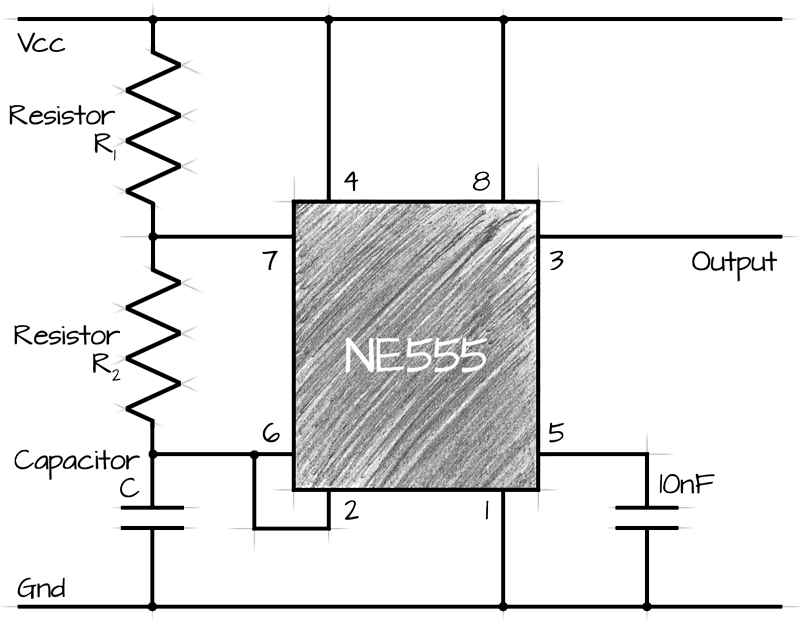
\includegraphics[width=80mm]{data/Ne555circuit.png}
		\caption[Verwendete Timerschaltung NE555 als Pulsquelle]{Verwendete Timerschaltung NE555 als Pulsquelle} %picture caption
		\label{fig:NE555}
	\end{center}
\end{figure}

$C= 1nF$\\
$R1: 200\Omega$\\
$R2:9 k\Omega$\\

Mit diesen Werten konnte nach dem Gleichrichter, bei einer Übertragungsdistanz von einer Standard-Platinen dicke, eine Leerlaufspannung von ca. 17V und ein Kurzschlussstrom ca. 300mA gemessen werden. Es gilt jedoch zu beachten, dass diese Werte ohne Last gemessen wurden. 

Da nun die Induktionsstufe funktioniert wird diese nun um die Ladeschaltung erweitert. Hier ergab sich folgendes Problem:

Die Eingangsspannung des Lade-Ic’s darf nicht mehr als 6.5 Volt betragen. Da die Receiverspule sich im inneren des Dojo’s befindet und dadurch nur eine sehr geringe Baugrösse besitzen darf, kann diese zwangsläufig keine grossen Leistungen erbringen. Dies bedeutet, dass akzeptabel Ladeströme nur mit genügend hohen Spannungen erzeugt werden können.

Um dies zu erzielen wurde versucht, einen Spannungsregler einzubauen, um den übertragenen Strom bei zuhalten, jedoch die Spannung zu begrenzen. Das Ergebnis davon war jedoch ziemlich bescheiden. Der so entstehende Energieverlust ist ziemlich gross und ausserdem kam es vereinzelt vor, dass der Lade ic trotzdem kaputt ging, da der Spannungsregler nicht sauber regelte. 

Die Ideale Lösung wäre natürlich einen geeigneteren Lade-Ic zu nehmen. Da jedoch die Validierung desjenigen bereits durchgeführt wurde und nicht genügend Zeit vorhanden war diesen erneut zu bestellen wurde sich entschieden die Transceiver Schaltung ein wenig anzupassen.

Dabei gibt es folgende Möglichkeiten. Man kann die Eingangsspannung absenken. Dies beeinflusst jedoch auch den Übertragenen Strom exponentiell, da einerseits eingangsseitig mit weniger Spannung auch weniger Strom durch die Spule fliess und andererseits auch der Leistungsstransistor nicht sauber durchgesteuert wird da dieser ebenfalls an der gleichen Versorgungsspannung hängt und somit sein Pulssignal beeinflusst. Die zweite Möglichkeit ist die Taktfrequenz verringern. Dadurch wird die Induzierte Spannung ebenfalls abgesengt was ebenfalls den Strom exponentiell beeinflusst. Die dritte Möglichkeit wäre die Übertragungsdistanz zu verringern. Da aber sichergestellt werden wollte, dass der Dojo-Boden dennoch eine gewisse Stabilität aufweisen sollte wurde diese Distanz der Platinendicke beigehalten.

Somit wurde die Schaltung lange ausgetestet um die beste Kombination zu erzielen. Das beste Resultat ergab die Kombination zwischen einer Taktfrequenz von ca 80kHz und einer Eingangs Spannung von 8.3V. Dies lässt sich damit erklären das leichtes Absenken der beiden Möglichkeiten den Strom nicht so stark beeinflusst. Des Weiteren wurde der Strombegrenzungswiderstand auf 1.5 Ohm verringert da sich die Eingangs Spannung verringert hat und ausserdem der Stromfluss durch die Spule damit erhöht wurde. 

Diese Anpassungen fielen ebenfalls zu Gunsten des Energiemanagements, jedoch ist dies eine stabile Variante für die ersten Prototypen. Durch die Anpassungen wird die überschüssige Energie in Form von Wärme an dem Transceiver Spule abgegeben. Die Test ergaben, dass so die Batterie bei einer Spannung von 4.7V mit 70mA geladen wird. Es ist ebenfalls möglich kurzzeitig mit einem höheren Strom zu laden, wenn die Eingangs Spannung nur geringfügig erhöht wird. (bis zu 120mA). Jedoch ist die Hitzeentwicklung hierbei so gross, dass nach einer gewissen Zeit die Übertragung zusammenbricht. Deshalb ist zu empfehlen die angegebenen Werte nicht zu überschreiten um eine dauernde Funktionalität zu gewährleisten.

Die Werte der oben beschriebenen angepassten Pulsschaltung sind folgende:\\
C: 1nF\\
R1: 200 Ohm\\
R2:9 kOhm\\

\subsubsection*{Optimierungsmöglichkeiten}\label{sec:optimierung}
Für nachfolgende Weiterentwicklungen der Ladestufe empfiehlt es sich, einen Lade-IC zu verwenden, welcher eine grössere Eingangsspannung verarbeiten kann. Bei einer Recherche wurde dieses Modell herausgesucht: AAAAAAAAAAAAAAA.

Desweiteren würde es sich Lohnen die Spulen zu optimieren. Die eingebauten Flachspulen sind zwar platzsparen, kommen jedoch aufgrund ihrer Bauform ziemlich schnell an ihr Leistungsmaximum. Hier würden sich solche Spulen sich empfehlen, wie sie z.B. auch in modernen elektrischen Zahnbürsten verwendet werden. Hierbei handelt es sich um zwei unterschiedlich grosse Ringspulen, von welchem die kleinere Tranceiver-Spule in der Ladeschaltung in die grössere Receiverspule  im Dojo gesteckt wird. Diese Ringspulen wären zwar ein wenig grösser, doch durch die grössere Bauform könnte die Ladeschaltung mit grösseren Strömen betrieben und damit auch der Dojo noch schneller geladen werden.